%https://www.integral-domain.org/lwilliams/Resources/TikzImg/semiregulartilings.tex
\documentclass[tikz]{standalone}

\begin{document}
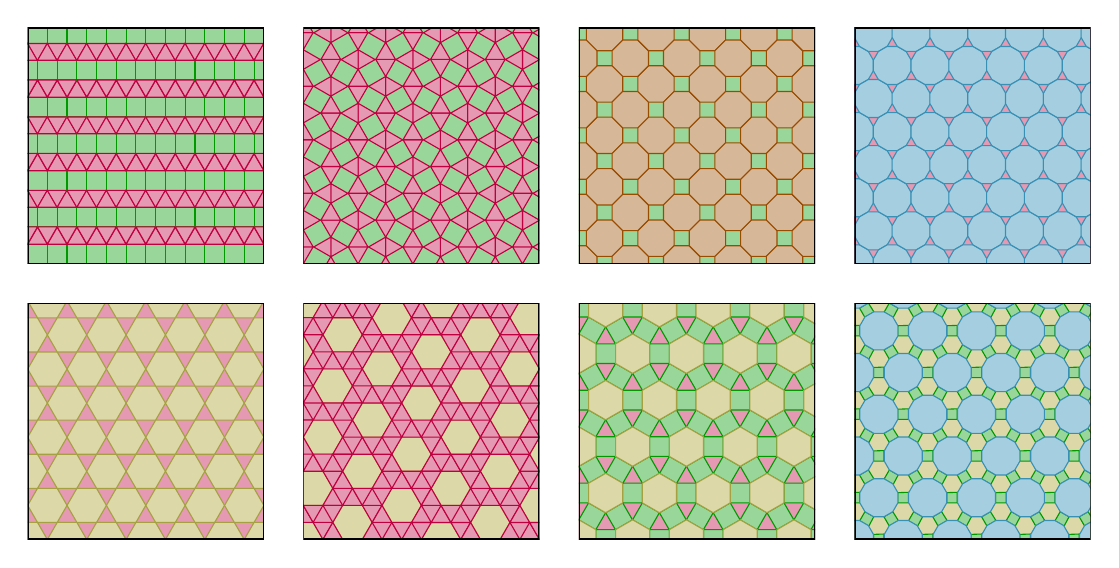
\begin{tikzpicture} 
    \begin{scope}
        \clip (0,0) rectangle (3,3);
        \foreach \c in {0,0.25,0.5,...,3}{
        \foreach \r in {0,1,2,3,4} {
            \begin{scope}[xshift=\c cm,yshift=\r*0.5cm + \r*0.5*0.866cm]
            \draw[green!60!black,fill=green!60!black!40](0,0) rectangle (0.25,0.25);
            \draw[purple,fill=purple!40](0,0.25) -- (0.25,0.25)--(0.5*0.25,0.25+0.25*0.866)--cycle;
            \draw[purple,fill=purple!40](0,0) -- (0.25,0)--(0.5*0.25,-0.25*0.866)--cycle;
            \end{scope}
            \begin{scope}[xshift=-0.125cm + \c cm,yshift=0.47cm + \r*0.5cm + \r*0.5*0.866cm]
            \draw[green!60!black,fill=green!60!black!40](0,0) rectangle (0.25,0.25);
            \draw[purple,fill=purple!40](0,0.25) -- (0.25,0.25)--(0.5*0.25,0.25+0.25*0.866)--cycle;
            \draw[purple,fill=purple!40](0,0) -- (0.25,0)--(0.5*0.25,-0.25*0.866)--cycle;
            \end{scope}
            }
        }
        \draw[thick] (0,0) rectangle (3,3);
    \end{scope}
    \begin{scope}[xshift=3.5cm]
     \clip (0,0) rectangle (3,3);
     \draw[green!60!black,fill=green!60!black!40](0,0) rectangle (3,3);
 
      \foreach \r in {0,1,2,3,4,5} {
      \foreach \c in {0,3,6,9,12} {
  
       \begin{scope}[xshift=\c*0.232cm, yshift=\r*0.68cm]
        \draw[purple,fill=purple!40](0,0) -- (60:0.25)--(120:0.25)--cycle;
        \draw[purple,fill=purple!40](0,0) -- (330:0.25)--(270:0.25)--cycle;
        \draw[purple,fill=purple!40](0,0) -- (210:0.25)--(270:0.25)--cycle;
        \draw[purple,fill=purple!40](60:0.25) -- (0,2*0.866*0.25)--(120:0.25)--cycle;
       \end{scope}
       \begin{scope}[xshift=0.35cm+\c*0.232cm, yshift=-0.34cm+\r*0.68cm]
        \draw[purple,fill=purple!40](0,0) -- (60:0.25)--(120:0.25)--cycle;
        \draw[purple,fill=purple!40](0,0) -- (330:0.25)--(270:0.25)--cycle;
        \draw[purple,fill=purple!40](0,0) -- (210:0.25)--(270:0.25)--cycle;
        \draw[purple,fill=purple!40](60:0.25) -- (0,2*0.866*0.25)--(120:0.25)--cycle;
       \end{scope}
      }
      }
    \draw[thick] (0,0) rectangle (3,3);
    \end{scope}
    \begin{scope}[xshift=7cm]
     \clip (0,0) rectangle (3,3);
     \draw[green!60!black,fill=green!60!black!40](0,0) rectangle (3,3);
     
     \foreach \c in {0,1,2,3,4}{
     \foreach \r in {0,1,2,3,4} {
      \begin{scope}[xshift=\c*0.653cm, yshift=\r*0.653cm]
      \draw[orange!60!black,fill=orange!60!black!40](22.5:0.25)--(67.5:0.25)--(112.5:0.25)--(157.5:0.25)--(202.5:0.25)--(247.5:0.25)--(292.5:0.25)--(337.5:0.25)--cycle;
      \end{scope}
      \begin{scope}[xshift=0.3265cm+\c*0.653cm, yshift=0.3265cm+\r*0.653cm]
      \draw[orange!60!black,fill=orange!60!black!40](22.5:0.25)--(67.5:0.25)--(112.5:0.25)--(157.5:0.25)--(202.5:0.25)--(247.5:0.25)--(292.5:0.25)--(337.5:0.25)--cycle;
      \end{scope}
 
     }
     }
     \draw[thick] (0,0) rectangle (3,3);
    \end{scope}
    \begin{scope}[xshift=10.5cm]
     \clip (0,0) rectangle (3,3);
     \draw[purple,fill=purple!40](0,0) rectangle (3,3);
     
     \foreach \c in {0,1,2,3,4,5,6,7}{
       \foreach \r in {0,2,4,6,8} {
        \begin{scope}[xshift=\c*0.48cm, yshift=\r*0.42cm]
        \draw[cyan!70!black,fill=cyan!70!black!40,rotate=15] (0:0.25)
          \foreach \a in {30,60,...,330} {
            --(\a:0.25)
          }
          --cycle;
        \end{scope}
       }
       \foreach \r in {1,3,5,7} {
        \begin{scope}[xshift=0.24cm+\c*0.48cm, yshift=\r*0.42cm]
        \draw[cyan!70!black,fill=cyan!70!black!40,rotate=15] (0:0.25)
          \foreach \a in {30,60,...,330} {
            --(\a:0.25)
          }
          --cycle;
        \end{scope}
       }
     }
     \draw[thick] (0,0) rectangle (3,3);
    \end{scope}
    \begin{scope}[yshift=-3.5cm]
     \clip (0,0) rectangle (3,3);
      \draw[purple,fill=purple!40](0,0) rectangle (3,3);
     
     \foreach \c in {0,1,2,...,6}{
     \foreach \r in {0,2,4,6} {
      \begin{scope}[xshift=\c*0.5cm, yshift=\r*0.433cm]
      \draw[yellow!60!black,fill=yellow!60!black!40] (0:0.25) -- (60:0.25) -- (120:0.25)--(180:0.25)--(240:0.25)--(300:0.25)--cycle;
      \end{scope}
     }
     \foreach \r in {1,3,5,7} {
      \begin{scope}[xshift=0.25cm+\c*0.5cm, yshift=\r*0.433cm]
      \draw[yellow!60!black,fill=yellow!60!black!40] (0:0.25) -- (60:0.25) -- (120:0.25)--(180:0.25)--(240:0.25)--(300:0.25)--cycle;
      \end{scope}
     }
     }
     \draw[thick] (0,0) rectangle (3,3);
    \end{scope}
    \begin{scope}[yshift=-3.5cm,xshift=3.5cm]
      \clip (0,0) rectangle (3,3);
      \draw[purple,fill=purple!40](0,0) rectangle (3,3);
     
     \foreach \c in {-2,-1,0,1,2,3,4,5}{
       \foreach \r in {-2,-1,0,1,2,3,4,5} {
 
        \begin{scope}[xshift= \c*0.625cm +\r*0.125cm, yshift=\c*0.2165cm + \r*0.65cm]
        \draw[yellow!60!black,fill=yellow!60!black!40] (0:0.25) -- (60:0.25) -- (120:0.25)--(180:0.25)--(240:0.25)--(300:0.25)--cycle;
        \draw[purple,fill=purple!40] (0:0.25) -- (300:0.25)--++(0.25,0)--cycle;
        \draw[purple,fill=purple!40,rotate= 60] (0:0.25) -- (300:0.25)--++(0.25,0)--cycle;
        \draw[purple,fill=purple!40,rotate= 120] (0:0.25) -- (300:0.25)--++(0.25,0)--cycle;
        \draw[purple,fill=purple!40,rotate= 180] (0:0.25) -- (300:0.25)--++(0.25,0)--cycle;
        \draw[purple,fill=purple!40,rotate= 240] (0:0.25) -- (300:0.25)--++(0.25,0)--cycle;
        \draw[purple,fill=purple!40,rotate= 300] (0:0.25) -- (300:0.25)--++(0.25,0)--cycle;
        \end{scope}
 
       }
 
     }
     \draw[thick] (0,0) rectangle (3,3);
\end{scope}
    \begin{scope}[yshift=-3.5cm,xshift=7cm]
     \clip (0,0) rectangle (3,3);
     \draw[purple,fill=purple!40](0,0) rectangle (3,3);
    \foreach \c in {-1,0,1,2,3,4,5}{
       \foreach \r in {0,2,4} {
        \begin{scope}[xshift=\c*0.683cm, yshift=\r*0.59cm]
         \draw[green!60!black,fill=green!60!black!40] (330:0.25) -- (30:0.25) -- ++(0.25,0)--++(0,-0.25)--cycle;
        \draw[green!60!black,fill=green!60!black!40,rotate=-60] (330:0.25) -- (30:0.25) -- ++(0.25,0)--++(0,-0.25)--cycle;
        \draw[green!60!black,fill=green!60!black!40,rotate=-120] (330:0.25) -- (30:0.25) -- ++(0.25,0)--++(0,-0.25)--cycle;
        \end{scope}
       }
        \foreach \r in {1,3,5} {
        \begin{scope}[xshift=0.34cm+\c*0.683cm, yshift=\r*0.59cm]
         \draw[green!60!black,fill=green!60!black!40] (330:0.25) -- (30:0.25) -- ++(0.25,0)--++(0,-0.25)--cycle;
        \draw[green!60!black,fill=green!60!black!40,rotate=-60] (330:0.25) -- (30:0.25) -- ++(0.25,0)--++(0,-0.25)--cycle;
        \draw[green!60!black,fill=green!60!black!40,rotate=-120] (330:0.25) -- (30:0.25) -- ++(0.25,0)--++(0,-0.25)--cycle;
        \end{scope}
       }
 
     }
     \foreach \c in {-1,0,1,2,3,4,5}{
       \foreach \r in {0,2,4} {
        \begin{scope}[xshift=\c*0.683cm, yshift=\r*0.59cm]
        \draw[yellow!60!black,fill=yellow!60!black!40] (30:0.25) -- (90:0.25) -- (150:0.25)--(210:0.25)--(270:0.25)--(330:0.25)--cycle;
 
        \end{scope}
       }
        \foreach \r in {1,3,5} {
        \begin{scope}[xshift=0.34cm+\c*0.683cm, yshift=\r*0.59cm]
        \draw[yellow!60!black,fill=yellow!60!black!40] (30:0.25) -- (90:0.25) -- (150:0.25)--(210:0.25)--(270:0.25)--(330:0.25)--cycle;
 
        \end{scope}
       }
 
     }
     \draw[thick] (0,0) rectangle (3,3);
\end{scope}
    \begin{scope}[yshift=-3.5cm,xshift=10.5cm]
    \clip (0,0) rectangle (3,3);
    \draw[yellow!60!black,fill=yellow!60!black!40](0,0) rectangle (3,3);
  
    \foreach \c in {-1,0,1,2,3,4,5}{
       \foreach \r in {0,2,4,6} {
        \begin{scope}[xshift=\c*0.62cm, yshift=\r*0.53cm]
        \draw[green!60!black,fill=green!60!black!40] (345:0.25) -- ++(0.134,0) -- ++(0,0.134) -- (15:0.25)--cycle;
        \draw[green!60!black,fill=green!60!black!40,rotate=-60] (345:0.25) -- ++(0.134,0) -- ++(0,0.134) -- (15:0.25)--cycle;
        \draw[green!60!black,fill=green!60!black!40,rotate=-120] (345:0.25) -- ++(0.134,0) -- ++(0,0.134) -- (15:0.25)--cycle;
 
        \end{scope}
       }
       \foreach \r in {1,3,5} {
        \begin{scope}[xshift=0.31cm+\c*0.62cm, yshift=\r*0.53cm]
        \draw[green!60!black,fill=green!60!black!40] (345:0.25) -- ++(0.134,0) -- ++(0,0.134) -- (15:0.25)--cycle;
        \draw[green!60!black,fill=green!60!black!40,rotate=-60] (345:0.25) -- ++(0.134,0) -- ++(0,0.134) -- (15:0.25)--cycle;
        \draw[green!60!black,fill=green!60!black!40,rotate=-120] (345:0.25) -- ++(0.134,0) -- ++(0,0.134) -- (15:0.25)--cycle;
 
        \end{scope}
       }
 
     }
     \foreach \c in {-1,0,1,2,3,4,5}{
       \foreach \r in {0,2,4,6} {
        \begin{scope}[xshift=\c*0.62cm, yshift=\r*0.53cm]
 
        \draw[cyan!70!black,fill=cyan!70!black!40,rotate=15] (0:0.25)
          \foreach \a in {30,60,...,330} {
            --(\a:0.25)
          }
          --cycle;
        \end{scope}
       }
       \foreach \r in {1,3,5} {
        \begin{scope}[xshift=0.31cm+\c*0.62cm, yshift=\r*0.53cm]
 
        \draw[cyan!70!black,fill=cyan!70!black!40,rotate=15] (0:0.25)
          \foreach \a in {30,60,...,330} {
            --(\a:0.25)
          }
          --cycle;
        \end{scope}
       }
 
     }
     \draw[thick] (0,0) rectangle (3,3);
     \end{scope}
 \end{tikzpicture}

\end{document}